\documentclass[11pt]{article}

\usepackage{amssymb,amsmath,amsfonts}
\usepackage{graphicx} % Include figure files
\usepackage{bm} % bold math

\textwidth40em
\oddsidemargin1em
\textheight135ex
\topmargin-10mm
%\parindent=0pt

\renewcommand{\baselinestretch}{1.3}
%\setlength{\parskip}{1em}

\pagestyle{plain}

\begin{document}

\thispagestyle{empty}

%\centerline{
\includegraphics[height=3cm]{LASAGNE-color-on-white_III.png}\hfill
\includegraphics[height=2.5cm]{FP7-gen-RGB.jpg}}
\centerline{
\includegraphics[height=4cm]{LASAGNE-color-on-white_III.png}}

\vskip1.5cm
\centerline{\LARGE\bf Software library for public use}

\vskip1cm
\centerline{\Large\bf Deliverable Number D3.5}

%\vskip0.5cm
%\centerline{\LARGE\bf Title of deliverable}
%\centerline{\LARGE\bf (with subtitle)}

\vskip2cm
\begin{center}
\begin{tabular}{||l|c||}%l
\hline\hline
{\bf Project Title:} & multi-LAyer SpAtiotemporal Generalized NEtworks\\
\hline
{\bf Project Acronym:} & LASAGNE\\
\hline
{\bf Contract Number:} & FP7-2012-STREP-318132\\
\hline\hline
\end{tabular}

\vskip2cm
\begin{tabular}{||l|l||}
\hline\hline
{\bf Deliverable Number:} & 3.5\\
\hline
{\bf Deliverable Title:} & Software library for public use\\
\hline
{\bf Deliverable Type:} & Report\\
\hline
{\bf Dissemination Level:} & PU (Public)\\
\hline
{\bf Deliverable Date:} & \today\hspace{6.8cm}\mbox{}\\
\hline
{\bf Contributing Workpackage:} & WP3 - Dynamical processes\\
\hline\hline
\end{tabular}
\end{center}

\vskip 1.5cm
\centerline{
\includegraphics[height=2.5cm]{FP7-gen-RGB.jpg}}

\setcounter{page}{0}
\newpage

\centerline{
\includegraphics[height=2.5cm]{logo.png}} 

\vspace{25pt}

multiNetX is a python package for the manipulation and study of
multilayer networks. The core of this package is a MultilayerGraph, a
class that inherits all properties from networkx.Graph().


multiNetX is a python package for the manipulation and study of
multilayer networks. The core of this package is a MultilayerGraph, a
class that inherits all properties from networkx.Graph().

This allows for:

\begin{itemize}
\itemsep1pt\parskip0pt\parsep0pt
\item
  Creating networks with weighted or unweighted links (only undirected
  networks are supported in this version)
\item
  Analysing the spectral properties of adjacency or Laplacian matrices
\item
  Visualizing dynamical processes by coloring the nodes and links
  accordingly
\end{itemize}

\pagebreak

\tableofcontents

\pagebreak

\section{How to install multiNetX}\label{how-to-install-multinetx}

multinetx does not need intallation. You simply download the source
files and save them into your file system. Then you have to add that
directory to your PYTHONPATH. In Unix/Linux you can do this by writting
in the terminal the following command:

\begin{verbatim}
export PYTHONPATH=path_to_your_python_libraries/multinetx:$PYTHONPATH
\end{verbatim}

\section{How to use multiNetX}\label{how-to-use-multinetx}

multiNetX is very easy to use. It is based on networkX package
(https://networkx.github.io/) which is written in pure python and make
use of the standard python packages numpy and scipy. Basic knowledge of
python2.7 as well as of those packages is required in order to
understand the following guide. A fundamental knowledge of network
theory is also required.

\paragraph{Import standard python packages for numerics and
plots}\label{import-standard-python-packages-for-numerics-and-plots}

\begin{verbatim}
import numpy as np
import matplotlib.pyplot as plt
%matplotlib inline
\end{verbatim}

\paragraph{Import the package
multiNetX}\label{import-the-package-multinetx}

\begin{verbatim}
import multinetx as mx
\end{verbatim}


\paragraph{Create three Erd``os- R'enyi networks with N nodes for each
layer}\label{create-three-erdos--renyi-networks-with-n-nodes-for-each-layer}

\begin{verbatim}
N = 5
g1 = mx.generators.erdos_renyi_graph(N,0.9,seed=218)
g2 = mx.generators.erdos_renyi_graph(N,0.9,seed=211)
g3 = mx.generators.erdos_renyi_graph(N,0.9,seed=208)
\end{verbatim}

\paragraph{Create an 3Nx3N lil sparse matrix. It will be used to
describe the layers
interconnection}\label{create-an-3nx3n-lil-sparse-matrix.-it-will-be-used-to-describe-the-layers-interconnection}

\begin{verbatim}
adj_block = mx.lil_matrix(np.zeros((N*3,N*3)))
\end{verbatim}

\paragraph{Define the type of interconnection among the layers (here we
use identity matrices thus connecting one-to-one the nodes among
layers)}\label{define-the-type-of-interconnection-among-the-layers-here-we-use-identity-matrices-thus-connecting-one-to-one-the-nodes-among-layers}

\begin{verbatim}
adj_block[0:  N,  N:2*N] = np.identity(N)    # L_12
adj_block[0:  N,2*N:3*N] = np.identity(N)    # L_13
adj_block[N:2*N,2*N:3*N] = np.identity(N)    # L_23

# use symmetric inter-adjacency matrix
adj_block += adj_block.T
\end{verbatim}

\paragraph{Create an instance of the MultilayerGraph
class}\label{create-an-instance-of-the-multilayergraph-class}

\begin{verbatim}
mg = mx.MultilayerGraph(list_of_layers=[g1,g2,g3],
                        inter_adjacency_matrix=adj_block)
\end{verbatim}

\paragraph{Weights can be added to the
edges}\label{weights-can-be-added-to-the-edges}

\begin{verbatim}
mg.set_edges_weights(intra_layer_edges_weight=2,
                     inter_layer_edges_weight=3)
\end{verbatim}

\section{Create a multiplex 2nd way}\label{create-a-multiplex-2nd-way}

\paragraph{Create an empty multiplex
network}\label{create-an-empty-multiplex-network}

\begin{verbatim}
mg = mx.MultilayerGraph()
\end{verbatim}

\paragraph{Add layers}\label{add-layers}

\begin{verbatim}
mg.add_layer(mx.generators.erdos_renyi_graph(N,0.9,seed=218))
mg.add_layer(mx.generators.erdos_renyi_graph(N,0.9,seed=211))
mg.add_layer(mx.generators.erdos_renyi_graph(N,0.9,seed=208))
\end{verbatim}

\paragraph{Create an instance of the MultilayerGraph
class}\label{create-an-instance-of-the-multilayergraph-class-1}

\begin{verbatim}
mg.layers_interconnect(inter_adjacency_matrix=adj_block)
\end{verbatim}

\paragraph{Weights can be added to the
edges}\label{weights-can-be-added-to-the-edges-1}

\begin{verbatim}
mg.set_edges_weights(intra_layer_edges_weight=2,
                     inter_layer_edges_weight=3)
\end{verbatim}

\section{Take some information for the multiplex
network}\label{take-some-information-for-the-multiplex-network}

\begin{verbatim}
print 'MultiNetX name:\n', mg.name ,'\n', mg.info(),'\n'

MultiNetX name:
gnp_random_graph(5,0.9) 
3-layer graph, intra_layer_edges:27, inter_layer_edges:15, number_of_nodes_in_layer:5  




print 'MultilayerGraph edges:',\
        '\n\n intra-layer edges: ',mg.get_intra_layer_edges(),\
        '\n\n inter-layer edges: ',mg.get_inter_layer_edges(),'\n' 

MultilayerGraph edges: 

 intra-layer edges:  [(0, 1), (0, 2), (0, 4), (1, 2), (1, 4), (2, 3), (2, 4), (3, 4),
 (5, 6), (5, 7), (5, 8), (5, 9), (6, 7), (6, 8), (6, 9), (7, 8), (7, 9), (8, 9), (10, 11), 
 (10, 12), (10, 13), (10, 14), (11, 12), (11, 13), (11, 14), (12, 13), (12, 14)] 

 inter-layer edges:  [(5, 0), (6, 1), (7, 2), (8, 3), (9, 4), (10, 0), (10, 5),
 (11, 1), (11, 6), (12, 2), (12, 7), (13, 3), (13, 8), (14, 4), (14, 9)] 




print 'intralayer edges of 1: ',mg.get_intra_layer_edges_of_layer(layer=0)
print 'intralayer edges of 2: ',mg.get_intra_layer_edges_of_layer(layer=1)
print 'intralayer edges of 3: ',mg.get_intra_layer_edges_of_layer(layer=2)

intralayer edges of 1:  [(0, 1), (0, 2), (0, 4), (1, 2), (1, 4), (2, 3), (2, 4), (3, 4)]
intralayer edges of 2:  [(5, 6), (5, 7), (5, 8), (5, 9), (6, 7), (6, 8), (6, 9), (7, 8), 
(7, 9), (8, 9)]
intralayer edges of 3:  [(10, 11), (10, 12), (10, 13), (10, 14), (11, 12), (11, 13), 
(11, 14), (12, 13), (12, 14)]
\end{verbatim}

\paragraph{A layer can be chosen: it is a networkx.Graph so it inherits
all of its
properties.}\label{a-layer-can-be-chosen-it-is-a-networkx.graph-so-it-inherits-all-of-its-properties.}

\begin{verbatim}
layer = 1
mg1 = mg.get_layer(layer-1)
print 'layer', layer, ' name is', mg1.name

layer 1  name is gnp_random_graph(5,0.9)



print 'Adjacency matrix:\n', \
        mx.adjacency_matrix(mg,weight=None).todense(),'\n'
print 'Adjacency matrix (weighted):\n', \
        mx.adjacency_matrix(mg,weight="weight").todense(),'\n'

Adjacency matrix:
[[0 1 1 0 1 1 0 0 0 0 1 0 0 0 0]
 [1 0 1 0 1 0 1 0 0 0 0 1 0 0 0]
 [1 1 0 1 1 0 0 1 0 0 0 0 1 0 0]
 [0 0 1 0 1 0 0 0 1 0 0 0 0 1 0]
 [1 1 1 1 0 0 0 0 0 1 0 0 0 0 1]
 [1 0 0 0 0 0 1 1 1 1 1 0 0 0 0]
 [0 1 0 0 0 1 0 1 1 1 0 1 0 0 0]
 [0 0 1 0 0 1 1 0 1 1 0 0 1 0 0]
 [0 0 0 1 0 1 1 1 0 1 0 0 0 1 0]
 [0 0 0 0 1 1 1 1 1 0 0 0 0 0 1]
 [1 0 0 0 0 1 0 0 0 0 0 1 1 1 1]
 [0 1 0 0 0 0 1 0 0 0 1 0 1 1 1]
 [0 0 1 0 0 0 0 1 0 0 1 1 0 1 1]
 [0 0 0 1 0 0 0 0 1 0 1 1 1 0 0]
 [0 0 0 0 1 0 0 0 0 1 1 1 1 0 0]] 

Adjacency matrix (weighted):
[[0 2 2 0 2 3 0 0 0 0 3 0 0 0 0]
 [2 0 2 0 2 0 3 0 0 0 0 3 0 0 0]
 [2 2 0 2 2 0 0 3 0 0 0 0 3 0 0]
 [0 0 2 0 2 0 0 0 3 0 0 0 0 3 0]
 [2 2 2 2 0 0 0 0 0 3 0 0 0 0 3]
 [3 0 0 0 0 0 2 2 2 2 3 0 0 0 0]
 [0 3 0 0 0 2 0 2 2 2 0 3 0 0 0]
 [0 0 3 0 0 2 2 0 2 2 0 0 3 0 0]
 [0 0 0 3 0 2 2 2 0 2 0 0 0 3 0]
 [0 0 0 0 3 2 2 2 2 0 0 0 0 0 3]
 [3 0 0 0 0 3 0 0 0 0 0 2 2 2 2]
 [0 3 0 0 0 0 3 0 0 0 2 0 2 2 2]
 [0 0 3 0 0 0 0 3 0 0 2 2 0 2 2]
 [0 0 0 3 0 0 0 0 3 0 2 2 2 0 0]
 [0 0 0 0 3 0 0 0 0 3 2 2 2 0 0]] 




fig = plt.figure()
ax = fig.add_subplot(111)
ax.imshow(mx.adjacency_matrix(mg,weight=None).todense(),
          origin='upper',interpolation='nearest',cmap=plt.cm.binary);
\end{verbatim}

\begin{figure}[htbp]
\centering
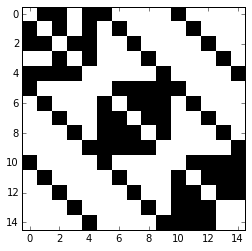
\includegraphics[width=0.5\textwidth]{output_35_0.png}
% \caption{png}
\end{figure}

\begin{verbatim}
print 'Laplacian matrix:\n',\
        mx.laplacian_matrix(mg,weight=None).todense(),'\n'
print 'Laplacian matrix (weighted):\n', \
        mx.laplacian_matrix(mg,weight="weight").todense(),'\n'

Laplacian matrix:
[[ 5 -1 -1  0 -1 -1  0  0  0  0 -1  0  0  0  0]
 [-1  5 -1  0 -1  0 -1  0  0  0  0 -1  0  0  0]
 [-1 -1  6 -1 -1  0  0 -1  0  0  0  0 -1  0  0]
 [ 0  0 -1  4 -1  0  0  0 -1  0  0  0  0 -1  0]
 [-1 -1 -1 -1  6  0  0  0  0 -1  0  0  0  0 -1]
 [-1  0  0  0  0  6 -1 -1 -1 -1 -1  0  0  0  0]
 [ 0 -1  0  0  0 -1  6 -1 -1 -1  0 -1  0  0  0]
 [ 0  0 -1  0  0 -1 -1  6 -1 -1  0  0 -1  0  0]
 [ 0  0  0 -1  0 -1 -1 -1  6 -1  0  0  0 -1  0]
 [ 0  0  0  0 -1 -1 -1 -1 -1  6  0  0  0  0 -1]
 [-1  0  0  0  0 -1  0  0  0  0  6 -1 -1 -1 -1]
 [ 0 -1  0  0  0  0 -1  0  0  0 -1  6 -1 -1 -1]
 [ 0  0 -1  0  0  0  0 -1  0  0 -1 -1  6 -1 -1]
 [ 0  0  0 -1  0  0  0  0 -1  0 -1 -1 -1  5  0]
 [ 0  0  0  0 -1  0  0  0  0 -1 -1 -1 -1  0  5]] 

Laplacian matrix (weighted):
[[12 -2 -2  0 -2 -3  0  0  0  0 -3  0  0  0  0]
 [-2 12 -2  0 -2  0 -3  0  0  0  0 -3  0  0  0]
 [-2 -2 14 -2 -2  0  0 -3  0  0  0  0 -3  0  0]
 [ 0  0 -2 10 -2  0  0  0 -3  0  0  0  0 -3  0]
 [-2 -2 -2 -2 14  0  0  0  0 -3  0  0  0  0 -3]
 [-3  0  0  0  0 14 -2 -2 -2 -2 -3  0  0  0  0]
 [ 0 -3  0  0  0 -2 14 -2 -2 -2  0 -3  0  0  0]
 [ 0  0 -3  0  0 -2 -2 14 -2 -2  0  0 -3  0  0]
 [ 0  0  0 -3  0 -2 -2 -2 14 -2  0  0  0 -3  0]
 [ 0  0  0  0 -3 -2 -2 -2 -2 14  0  0  0  0 -3]
 [-3  0  0  0  0 -3  0  0  0  0 14 -2 -2 -2 -2]
 [ 0 -3  0  0  0  0 -3  0  0  0 -2 14 -2 -2 -2]
 [ 0  0 -3  0  0  0  0 -3  0  0 -2 -2 14 -2 -2]
 [ 0  0  0 -3  0  0  0  0 -3  0 -2 -2 -2 12  0]
 [ 0  0  0  0 -3  0  0  0  0 -3 -2 -2 -2  0 12]] 




fig = plt.figure()
ax = fig.add_subplot(111)
ax.imshow(mx.laplacian_matrix(mg,weight=None).todense(),
          origin='upper',interpolation='nearest',cmap=plt.cm.binary);
\end{verbatim}

\begin{figure}[htbp]
\centering
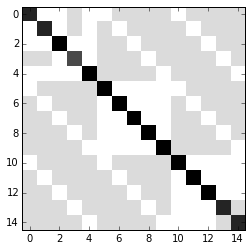
\includegraphics[width=0.5\textwidth]{output_37_0.png}
% \caption{png}
\end{figure}

\begin{verbatim}
print 'Laplacian spectrum:\n', \
        mx.laplacian_spectrum(mg,weight="weight"),'\n'

Laplacian spectrum:
[  7.29267473e-15   6.55428082e+00   8.90511420e+00   9.00000000e+00
   9.00000000e+00   9.22799813e+00   1.00000000e+01   1.51991214e+01
   1.73414836e+01   1.77720019e+01   1.90000000e+01   1.90000000e+01
   1.90000000e+01   1.90000000e+01   1.90000000e+01] 
\end{verbatim}

\section{Plot Multiplex}\label{plot-multiplex}

\subsubsection{Edge colored nertwork (no inter-connected
layers)}\label{edge-colored-nertwork-no-inter-connected-layers}

\subparagraph{Create a multiplex network with three random
layers}\label{create-a-multiplex-network-with-three-random-layers}

\begin{verbatim}
mg = mx.MultilayerGraph()


N = 50
mg.add_layer(mx.generators.erdos_renyi_graph(N,0.07,seed=218))
mg.add_layer(mx.generators.erdos_renyi_graph(N,0.07,seed=211))
mg.add_layer(mx.generators.erdos_renyi_graph(N,0.07,seed=208))
\end{verbatim}

\subparagraph{Set weights to the edges}\label{set-weights-to-the-edges}

\begin{verbatim}
mg.set_intra_edges_weights(layer=0,weight=1)
mg.set_intra_edges_weights(layer=1,weight=2)
mg.set_intra_edges_weights(layer=2,weight=3)


fig = plt.figure(figsize=(15,5))
ax1 = fig.add_subplot(121)
ax1.imshow(mx.adjacency_matrix(mg,weight='weight').todense(),
          origin='upper',interpolation='nearest',cmap=plt.cm.jet_r)
ax1.set_title('supra adjacency matrix')

ax2 = fig.add_subplot(122)
ax2.axis('off')
ax2.set_title('edge colored network')
pos = mx.get_position(mg,mx.fruchterman_reingold_layout(mg.get_layer(0)),
                      layer_vertical_shift=0.2,
                      layer_horizontal_shift=0.0,
                      proj_angle=47)
mx.draw_networkx(mg,pos=pos,ax=ax2,node_size=50,with_labels=False,
                 edge_color=[mg[a][b]['weight'] for a,b in mg.edges()],
                 edge_cmap=plt.cm.jet_r)
plt.show()
\end{verbatim}

\begin{figure}[htbp]
\centering
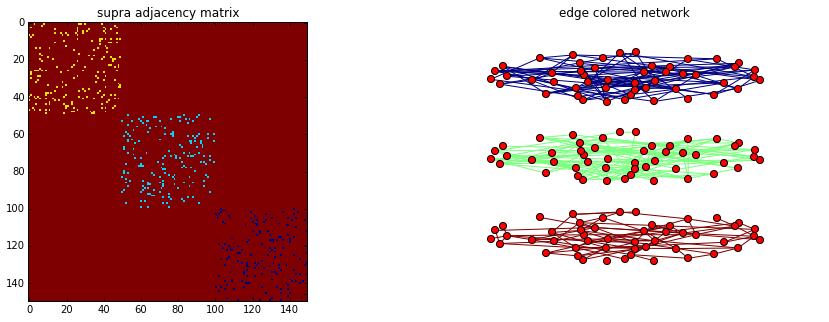
\includegraphics[width=\textwidth]{output_46_0.png}
% \caption{png}
\end{figure}

\subsubsection{Regular interconnected
multiplex}\label{regular-interconnected-multiplex}

\subparagraph{Define the type of interconnection between the
layers}\label{define-the-type-of-interconnection-between-the-layers}

\begin{verbatim}
adj_block = mx.lil_matrix(np.zeros((N*3,N*3)))

adj_block[0:  N,  N:2*N] = np.identity(N)    # L_12
adj_block[0:  N,2*N:3*N] = np.identity(N)    # L_13
#adj_block[N:2*N,2*N:3*N] = np.identity(N)    # L_23
adj_block += adj_block.T


mg.layers_interconnect(inter_adjacency_matrix=adj_block)

mg.set_edges_weights(inter_layer_edges_weight=4)

mg.set_intra_edges_weights(layer=0,weight=1)
mg.set_intra_edges_weights(layer=1,weight=2)
mg.set_intra_edges_weights(layer=2,weight=3)


fig = plt.figure(figsize=(15,5))
ax1 = fig.add_subplot(121)
ax1.imshow(mx.adjacency_matrix(mg,weight='weight').todense(),
          origin='upper',interpolation='nearest',cmap=plt.cm.jet_r)
ax1.set_title('supra adjacency matrix')

ax2 = fig.add_subplot(122)
ax2.axis('off')
ax2.set_title('regular interconnected network')
pos = mx.get_position(mg,mx.fruchterman_reingold_layout(mg.get_layer(0)),
                      layer_vertical_shift=1.4,
                      layer_horizontal_shift=0.0,
                      proj_angle=7)
mx.draw_networkx(mg,pos=pos,ax=ax2,node_size=50,with_labels=False,
                 edge_color=[mg[a][b]['weight'] for a,b in mg.edges()],
                 edge_cmap=plt.cm.jet_r)
plt.show()
\end{verbatim}

\begin{figure}[htbp]
\centering
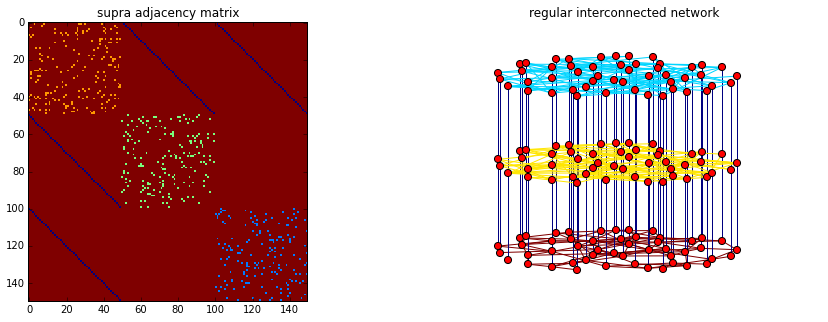
\includegraphics[width=\textwidth]{output_51_0.png}
% \caption{png}
\end{figure}

\subsubsection{General multiplex}\label{general-multiplex}

\begin{verbatim}
adj_block = mx.lil_matrix(np.zeros((N*4,N*4)))

adj_block[0  :  N ,   N:2*N] = np.identity(N)   # L_12
adj_block[0  :  N , 2*N:3*N] = np.random.poisson(0.005,size=(N,N))   # L_13
adj_block[0  :  N , 3*N:4*N] = np.random.poisson(0.006,size=(N,N))   # L_34
adj_block[3*N:4*N , 2*N:3*N] = np.random.poisson(0.008,size=(N,N))   # L_14
adj_block += adj_block.T
adj_block[adj_block>1] = 1
\end{verbatim}

\subparagraph{Add one more layer}\label{add-one-more-layer}

\begin{verbatim}
mg.add_layer(mx.generators.erdos_renyi_graph(N,0.1,seed=218))


mg.layers_interconnect(inter_adjacency_matrix=adj_block)

mg.set_edges_weights(inter_layer_edges_weight=5)

mg.set_intra_edges_weights(layer=0,weight=1)
mg.set_intra_edges_weights(layer=1,weight=2)
mg.set_intra_edges_weights(layer=2,weight=3)
mg.set_intra_edges_weights(layer=3,weight=4)


fig = plt.figure(figsize=(15,5))
ax1 = fig.add_subplot(121)
ax1.imshow(mx.adjacency_matrix(mg,weight='weight').todense(),
          origin='upper',interpolation='nearest',cmap=plt.cm.jet_r)
ax1.set_title('supra adjacency matrix')

ax2 = fig.add_subplot(122)
ax2.axis('off')
ax2.set_title('general multiplex network')
pos = mx.get_position(mg,mx.fruchterman_reingold_layout(mg.get_layer(0)),
                      layer_vertical_shift=.4,
                      layer_horizontal_shift=1.2,
                      proj_angle=.2)
mx.draw_networkx(mg,pos=pos,ax=ax2,node_size=50,with_labels=False,
                 edge_color=[mg[a][b]['weight'] for a,b in mg.edges()],
                 edge_cmap=plt.cm.jet_r)
plt.show()
\end{verbatim}

\begin{figure}[htbp]
\centering
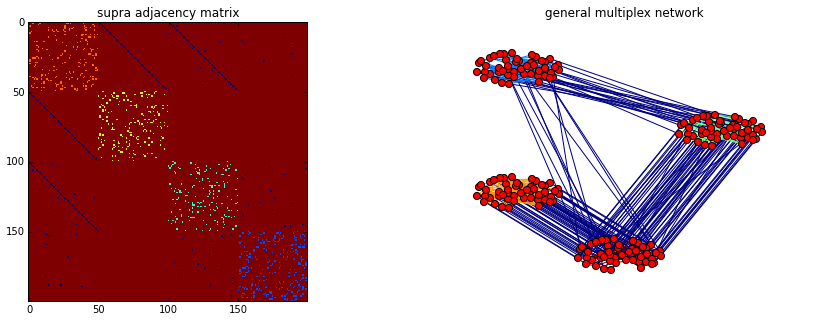
\includegraphics[width=\textwidth]{output_57_0.png}
% \caption{png}
\end{figure}



\section{Dynamical processes on top of multiplex networks}

\paragraph{Import libraries}\label{import-libraries}

\begin{verbatim}
import numpy as np
import matplotlib.pylab as plt

import multinetx as mx

from scipy.integrate import ode
\end{verbatim}

\paragraph{The Mimura-Murray ecological
model}\label{the-mimura-murray-ecological-model}

\begin{verbatim}
def mimura_murray_duplex(t, y0, G):
    f = y0.copy()    
    u = y0[:G.N] # activator
    v = y0[G.N:] # inhibitor    
    sum_lapl_u = G.diff[0] * u * G.lapl[0:G.N,0:G.N]   
    sum_lapl_v = G.diff[1] * v * G.lapl[G.N:2*G.N,G.N:2*G.N]    
    # activator
    f[:G.N] = ( (G.a + G.b * u - u * u) / G.c - v) * u + sum_lapl_u
    # inhibitor   
    f[G.N:] = (u - 1.0 - G.d * v) * v + sum_lapl_v
    return f 
\end{verbatim}

\paragraph{Define the integrate
method}\label{define-the-integrate-method}

\begin{verbatim}
def integrate(G, dt=0.5, tmax=200, method='dopri5', store_solution=True):
    '''This function integrates the MM model'''
    ## Setup the integrator 
    t0 = 0.0
    sol = [G.species]
    solver = ode(G.rhs).set_f_params(G)
    int_pars = dict(atol=1E-8, rtol=1E-8, first_step=1E-2,
                    max_step=2E1, nsteps=2E4)
    solver.set_integrator(method,**int_pars)
    solver.set_initial_value(G.species,t0)
    ## Integrate the system    
    while solver.successful() and solver.t < tmax:
        solver.integrate(solver.t+dt)
        sol.append(solver.y)
    return np.array(sol)
\end{verbatim}

\paragraph{Create the activator-inhibitor
multiplex}\label{create-the-activator-inhibitor-multiplex}

\begin{verbatim}
G = mx.MultilayerGraph()


N = 350
G.add_layer(mx.barabasi_albert_graph(n=N, m=5,   seed=812))   # activators
G.add_layer(mx.barabasi_albert_graph(n=N, m=200, seed=812))   # inhibitors
\end{verbatim}

\paragraph{Laplacian matrices of the
multiplex}\label{laplacian-matrices-of-the-multiplex}

\begin{verbatim}
G.lapl = (-1.0) * mx.laplacian_matrix(G,weight=None)
\end{verbatim}

\paragraph{Right-hand-side of the Mimura-Murray
model}\label{right-hand-side-of-the-mimura-murray-model}

\begin{verbatim}
G.rhs = mimura_murray_duplex
\end{verbatim}

\paragraph{Define the parameters of the model (They correspond to the
uniform steady
state)}\label{define-the-parameters-of-the-model-they-correspond-to-the-uniform-steady-state}

\begin{verbatim}
G.a = 35.0
G.b = 16.0
G.c = 9.0
G.d = 0.4


G.N = G.get_number_of_nodes_in_layer() 
G.diff = [0.12, 0.12]  
\end{verbatim}

\paragraph{Initial conditions and
perturbation}\label{initial-conditions-and-perturbation}

\begin{verbatim}
activators = np.empty(G.N,dtype=np.double)
inhibitors = np.empty(G.N,dtype=np.double)
activators[:] = 5.0
inhibitors[:] = 10.0
activators[10] += 10E-5
G.species = np.concatenate((activators,inhibitors),axis=0)
\end{verbatim}

\paragraph{Integrate the system}\label{integrate-the-system}

\begin{verbatim}
sol = integrate(G,dt=0.5,tmax=200,method='dopri5')
\end{verbatim}

\paragraph{Sort the solution according to decreasing degree of the
activator
layer}\label{sort-the-solution-according-to-decreasing-degree-of-the-activator-layer}

\begin{verbatim}
deg_act = G.get_layer(0).degree().values()
sdeg_act = np.argsort(deg_act)[::-1]
sdeg_sol = np.append(sdeg_act,G.N+sdeg_act)
ssol = sol[:,sdeg_sol]


def plot_sol(ax, insol, NN, t=0):
    ax.plot(insol[t],':',color='green',lw=1.1,alpha=1)
    sc = ax.scatter(np.arange(NN),insol[t],
                    c=insol[t],s=25,marker='o',lw=1.2,
                    vmin=min(insol[t]),vmax=max(insol[t]),
                    cmap=plt.cm.YlOrBr)
    ax.set_xlim(-5,NN)


%matplotlib inline
\end{verbatim}

\paragraph{Development of Turing pattern (activator layer is
shown)}\label{development-of-turing-pattern-activator-layer-is-shown}

\begin{verbatim}
sol_act = ssol[:,:G.N]

fig = plt.figure()
ax1 = fig.add_subplot(221)
ax1.set_ylabel(r'$u_i$')
ax1.set_title(r'$t=0$')
ax1.set_ylim(0,10)
ax1.set_xticks([])
plot_sol(ax1,sol_act,G.N,t=0)

ax2 = fig.add_subplot(222)
ax2.set_ylabel(r'$v_i$')
ax2.set_title(r'$t=18$')
ax2.set_ylim(0,10)
ax2.set_xticks([])
plot_sol(ax2,sol_act,G.N,t=18)

ax3 = fig.add_subplot(223)
ax3.set_xlabel(r'$i$')
ax3.set_ylabel(r'$v_i$')
ax3.set_title(r'$t=21$')
ax3.set_ylim(0,10)
plot_sol(ax3,sol_act,G.N,t=21)

ax4 = fig.add_subplot(224)
ax4.set_xlabel(r'$i$')
ax4.set_ylabel(r'$v_i$')
ax4.set_title(r'$t=400$')
ax4.set_ylim(0,10)
plot_sol(ax4,sol_act,G.N,t=400)

plt.show()
\end{verbatim}

\begin{figure}[htbp]
\centering
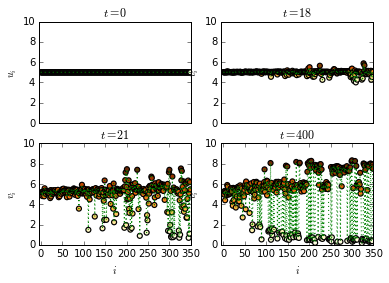
\includegraphics[width=0.7\textwidth]{multiplex_turing_patterns_25_0.png}
% \caption{png}
\end{figure}

\paragraph{Turing pattern shown in activator and inhibitor
layer}\label{turing-pattern-shown-in-activator-and-inhibitor-layer}

\begin{verbatim}
sol_act = ssol[:,:G.N]
sol_inh = ssol[:,G.N:]
tsnap = 400

fig = plt.figure()
ax1 = fig.add_subplot(211)
ax1.set_ylabel(r'$u_i$')
ax1.set_ylim(0,10)
plot_sol(ax1,sol_act,G.N,t=tsnap)

ax2 = fig.add_subplot(212)
ax2.set_xlabel(r'$i$')
ax2.set_ylabel(r'$v_i$')
ax2.set_ylim(7.5,11.1)
plot_sol(ax2,sol_inh,G.N,t=tsnap)

plt.show()
\end{verbatim}

\begin{figure}[h!]
\centering
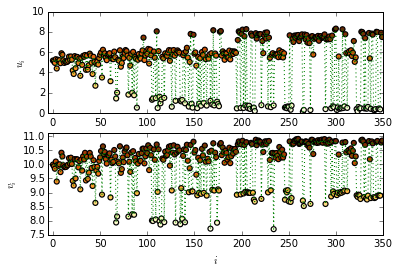
\includegraphics[width=0.7\textwidth]{multiplex_turing_patterns_27_0.png}
% \caption{png}
\end{figure}


\pagebreak

\section{Copyright}\label{copyright}

Copyright \textcopyright~ 2013-2019, Nikos E Kouvaris


\vspace{10pt}
\noindent Each file in this folder is part of the multiNetX package.

\vspace{10pt}
\noindent multiNetX is part of the deliverables of the LASAGNE project
(multi-LAyer SpAtiotemporal Generalized NEtworks),
EU/FP7-2012-STREP-318132
(http://complex.ffn.ub.es/\textasciitilde{}lasagne/)

\vspace{10pt}
\noindent multiNetX is free software: you can redistribute it and/or modify it
under the terms of the GNU General Public License as published by the
Free Software Foundation, either version 3 of the License, or (at your
option) any later version.

\vspace{10pt}
\noindent multiNetX is distributed in the hope that it will be useful, but WITHOUT
ANY WARRANTY; without even the implied warranty of MERCHANTABILITY or
FITNESS FOR A PARTICULAR PURPOSE. See the GNU General Public License for
more details.

\vspace{10pt}
\noindent You should have received a copy of the GNU General Public License along
with this program. If not, see http://www.gnu.org/licenses/.



\end{document} 